% Template for PLoS
% Version 1.0 January 2009
%
% To compile to pdf, run:
% latex plos.template
% bibtex plos.template
% latex plos.template
% latex plos.template
% dvipdf plos.template

\documentclass[10pt]{article}
\usepackage{amsmath}
\usepackage{amssymb}
\usepackage{graphicx}
\usepackage{color} % for revision purposes only, may be not present in the final file
% cite package, to clean up citations in the main text. Do not remove.
\usepackage{cite}
\usepackage{color}
\usepackage{indentfirst} %% L: in order to indent the first paragraph of each section
\usepackage{url} %% L: in order to include nice urls
% Use doublespacing - comment out for single spacing
%\usepackage{setspace}
%\doublespacing

\topmargin 0.0cm
\oddsidemargin 0.5cm
\evensidemargin 0.5cm
\textwidth 16cm
\textheight 21cm

\usepackage[labelfont=bf,labelsep=period,justification=raggedright]{caption}

\bibliographystyle{plos2009}% 


\makeatletter
\renewcommand{\@biblabel}[1]{\quad#1.}
\makeatother


% Leave date blank
\date{}

\pagestyle{myheadings}
%% ** EDIT HERE **


%% ** EDIT HERE **
%% PLEASE INCLUDE ALL MACROS BELOW

%% END MACROS SECTION

\begin{document}

% Title must be 150 characters or less
\begin{flushleft}
{\Large
\textbf{Spatio-temporal Dynamics of Foot-and-mouth Disease Virus in South America}
}
% Insert Author names, affiliations and corresponding author email.
\\
Luiz Max Fagundes de Carvalho$^{1\ast}$,
Nuno Faria$^{2}$,
Guy Baele$^{2}$,
Andres M. Perez$^{3}$,
Philippe Lemey$^{2}$,
Waldemir de Castro Silveira$^{1}$
\\
\bf{1} Pan American Center for Foot-and-Mouth Disease (PAHO/WHO), Duque de Caxias, Rio de Janeiro, Brazil
\\
\bf{2} Department of Microbiology and Immunology, Katholieke Universiteit Leuven, Leuven, Belgium
\\
\bf{3} Center for Animal Disease Modeling and Surveillance, University of California at Davis, Davis, United States of America
\\
$\ast$ E-mail: Corresponding lcarvalho@paho.org
\end{flushleft}

% Please keep the abstract between 250 and 300 words
\section*{Abstract}

JUST IN THE END :)\\


Key-words: Phylogeography, foot-and-mouth disease virus, South America, animal trade, BEAST.
\section*{Introduction}
\indent Foot-and-mouth disease virus (FMDV) is a rapidly evolving picornavirus, causative agent of the most important disease of domestic and wild cloven-hoofed animals, foot-and mouth disease (FMD) \cite{review}. FMD is endemic in several regions of South America, and in recent years, the circulation of three of the seven FMDV serotypes C, A and O has been reported in the continent, the later two being the most prevalent. Serotypes A and O show different  geographic distribution, with O being more prevalent in endemic Andean areas \cite{andean} and A being responsible for sporadic emergences in the Southern cone \cite{Perez2001,Malirat2012
}.\\
\indent FMDV is likely to have been introduced in South America in the early days of European colonization. Large outbreaks, however, were not observed until the end of 19th century. By the 1970's, FMD was widespread in South America, with occurrence of multiple sub-types \cite{Saraiva2003} in large-scale outbreaks. As a consequence of the improving knowledge about disease ecosystems accumulated by the national programmes, the Hemispheric Plan for the Eradication of FMD (PHEFA) was launched in 1987. PHEFA was elaborated and signed by South American countries as a continent-wide programme to strenghten national infra-structures, control animal trade and improve diagnostic and epidemiological investigation capabilities \cite{review_eradication}. The main objective is to create and maintain FMD-free areas, thus improving the availability of meat, milk and other economically important livestock products \cite{Saraiva2003,Saraiva2004,review_eradication,combining}. Considerable success has been achieved over the 
past years, with substantial reduction of FMD incidence in the late 1990's. Nevertheless, episodic outbreaks in 2001, 2005 and 2011 in previously free areas represented a serious setback to PHEFA, which was devised to fulfill its goals by 2010 \cite{Saraiva2003,Saraiva2004}.\\
\indent The generally accepted solution to the problem of FMD eradication is two fold: by one side, the promotion of massive vaccination programmes \cite{vaccinationSA} and strenghtening of co-operation between national governments and the private sector; by the other, the development of better veterinary surveillance systems. In this last matter, phylogenetic analyses have proved useful in unraveling transmission pathways \cite{cottam2008} and providing insight into the processes that drive reemergence \cite{combining}. In the South American ecotone, the molecular evolution of FMDV has been subject of several studies along the years \cite{Perez2001,Malirat2007,andean,Malirat2011,Maradei2013}. These studies have played an important role in understanding the (re-)emergence pattern of FMDV, allowing for inference on the origin and evolutionary history of emerging viral strains \cite{topotypes,Perez2001}. Together with vaccine matching and MAb profiling studies \cite{Maradei2011}, phylogenetic analyses are a 
powerful tool to evaluate control programmes and guide vaccine formulation \cite{Maradei2011,Maradei2013}.\\
\indent However, to allow epidemiological inference, phylogenetic evidence has still to be combined with other pieces of information, such as animal trade patterns, farming practices and herd density and composition. As pointed out by Di Nardo, Knowles \&  Paton (2011) \cite{combining}, this joint evaluation of information from different sources is usually done outside of a unified quantitative framework, in a qualitative fashion. As the authors state, Bayesian phylogeography may offer the framework to combine multiple sources of information in order to understand the spatio-temporal dynamics of FMDV and perform evolutionary hypothesis testing.\\
\indent The increased availability of molecular sequences with known date and location of sampling has fostered the development of new methods to integrate epidemiological and environmental data in order to reconstruct pathogen population dynamics and test evolutionary hypotheses \cite{MEP,grenfell}. Most notably, Bayesian phylogeography, introduced by Lemey et al. (2009) \cite{roots}, has been successfully applied to study FMDV patterns of spread as well as trace spatial  origins of FMD epidemics \cite{Carvalho2012,bulgaria,phymal}.\\
\indent In this study we apply state-of-art Bayesian Phylogeography methods, implemented within the BEAST \cite{BEAST} package, to address the evolutionary dynamics of serotypes A and O in South America, both in space and in time. This full probabilistic framework allows for incorporating multiple sources of information in order to test hypothesis about viral dispersal, while naturally accommodating uncertainty \cite{roots,towards}. We use BEAST to build time-structured phylogenies and the Skygrid model to reconstruct past population dynamics, to which we overlay vaccination and serotype-specific notification data. Moreover, we use data on livestock trade and geographical distances as predictors for viral spatial diffusion and use recently developed methods to accurately calculate marginal likelihoods for each predictor. Finally, we offer an appreciation of the statistical hurdles that may be caused by biased geographic sampling, and propose ways to ameliorate their effects.\\
% Results and Discussion can be combined.\\
\section*{Results}
\subsection*{Phylogenetic Analysis and Demographic Reconstruction}
\indent In this study, we analyzed all publicly available VP1 (1D) sequences for serotypes A and O in South America (131 and 167 sequences, respectively) from a Bayesian phylogenetic point of view. The BEAST \cite{BEAST} package was used to build time-structured phylogenies for each serotype, as well as select the best combination of tree (coalescent) prior and molecular clock model. The results of this last analysis (Table S1) allowed for decisive rejection of the constant population assumption (A: BF= 11; O: BF= 21.1). Interestingly, best fit molecular clock models were different for the two serotypes (O: exponential, A: lognormal, Table S1), suggesting different evolutionary dynamics. Moreover, a `temporal signal' test (see Methods) showed that both serotypes present substantial temporal information contained in the sequences (A:BF=310; O:BF=348).\\
\indent The maximum clade credibility (MCC) tree estimated for serotype A (Figure~\ref{fig:Atree}) shows a time to most common recent ancestor (TMRCA) of around 75 years, placing the origin of the circulating strains in the early years of the 1920's decade. Also, the mutation rate was estimated around $4$ x $10^{-3}$ substitutions/site/year. Figure~\ref{fig:Atree} shows that sequences from the same location do not present a tendency to form monophyletic clades, showing considerable interspersing, what suggests viral flow between countries (see also Spatial Signal below).\\
\indent Figure~\ref{fig:Otree} presents the estimated MCC tree for serotype O. The same interspersing trend can be noticed, with Ecuador and Colombia showing several interleaved clades. \\
\indent The Skygrid results show strikingly different dynamical behaviors for the two serotypes, with serotype O exhibiting considerable more oscillation over time, and a diversity peak occurring in late years of the 1990 decade. Serotype A exhibits a more stable behavior over most of the 20th century, with most variation occurring within the temporal sampling interval, mainly in the last years of the 2000 decade.\\
\subsection*{Spatial Dynamics of FMDV in South America}
\begin{itemize}
 \item BaTS
 \item MJ and BSSVS
 \item shared vs separated
 \item Regions
\end{itemize}

\subsection*{Sampling Bias Assessment}
\section*{Discussion}
% You may title this section "Methods" or "Models".
% "Models" is not a valid title for PLoS ONE authors. However, PLoS ONE
% authors may use "Analysis"
\indent Informing the rates with livestock trade contributes to ameliorate the bias introduced by unbalanced sampling in the sense that it allows for an external source of information to be incorporated \cite{Faria2012}. Moreover, our results suggest that \ldots\\
\indent \textcolor{red}{Skygrid is specially suited to detect slight but meaningful variation in population effective sizes, allowing for more precise epidemiological inference}.\\
\indent REMEMBER TO DISCUSS SHARED VERSUS SEPARATED ANALYSES.\\
\section*{Methods}
\subsection{Data}
\indent In order to study the spatio-temporal spread dynamics of FMDV within South America we compiled the largest database of 1D (VP1) gene sequences to date for serotypes A and O. We retrieved all 1D (VP1) genomic sequences available from the National Center for Biotechnology Information (NCBI, \url{ http://www.ncbi.nlm.nih.gov/}) for which there was information on country and year of isolation.  This resulted in 131 sequences (eight countries) for serotype A and 167 sequences (nine countries) for serotype O, covering time spans of 55 (1955-2008) and 16 (1994-2010) years, respectively (see Text S1 for details).\\
\indent Data on animal trade were obtained from the FAO database (\url{http://faostat.fao.org/}). We retrieved data on the detailed trade matrix for cattle, pigs and sheep (live animals) covering the period from 1986 to 2009, for each of the nine countries. Serotype-specific outbreak notifications were obtained from FMD Bioportal (\url{http://fmdbioportal.ucdavis.edu:8080/}).\\
\subsection{Phylogenetic Analysis}
\indent First, we use hierarchical likelihood model selection, as implemented in the package jModeltest 0.1.1 \cite{jmodel}, to select the best nucleotide substitution model for each data set. This analysis yielded the general time reversible (GTR) model with a discretized gamma distributed across-site rate variation and a proportion of invariant sites (GTR+I+$\Gamma_{4}$) model as the best fit for both data sets.\\
\indent We conducted a computationally intensive Bayesian model selection procedure, using recently developed path sampling (PS) and stepping stone sampling (SS) methods \cite{Baele2012a}[MORE ``BAELES'' HERE?] to calculate marginal likelihoods and Bayes factors (BF) for several combinations of tree priors (skyride and constant population) and molecular clocks (uncorrelated log-normal and exponential distributions) for each data set. The results of this study can be found in Table S1. Next, we employ high-end Bayesian coalescent-based methods to build time-structured phylogenies for the two serotypes and gain insight into the past population dynamics of the virus and make inference about the time to most recent common ancestor (TMRCA) using the BEAST \cite{BEAST} package, along with the BEAGLE \cite{beagle} library to gain computational efficiency.\\
\subsection{Quantifying temporal and spatial signal} 
\indent To assess the ``temporal signal'' for each serotype, we took the approach of Faria et al (2012) \cite{Faria2012} and compared the marginal likelihoods of a ``dated tips'' model and a contemporaneous tips model by calculating Bayes factors (BF) \cite{Suchard2001,KassRaftery1995} (see Spatial Model Selection for details). We followed Kass and Raftery (1995) \cite{KassRaftery1995} and considered BF$>3$ to be indicator of decisive support for the hypothesis of temporal structure.\\
\indent Spatial signal was quantified using Bayesian tip-association tests, implemented through the BaTS software package\cite{bats}. Each sequence was assigned to its country of origin and we computed association index (AI) and parsimony score (PI). Using a subset of 1000 samples from the posterior distribution of topologies, we obtained a null distribution for each statistic, against which the observed indexes were compared and significance was assessed. Additionally, we computed the so-called monophyletic clade (MC) size for each state (country), as a local indicator of phylogeny-trait association for each state.\\
\subsection{Temporal Dynamics}
\indent We apply the recently developed Skygrid coalescent model \cite{skygrid} in order to reconstruct the past population dynamics for both serotypes and then overlay the results to serotype-specific outbreak notifications.\\
\indent Skygrid is a nonparametric coalescent-based method that uses a Gaussian Markov Random Field (GMRF) prior to obtain smooth estimates for effective population size trajectories over time \ldots [NUNO'S SHARE]
\subsection{Spatial Analysis}
\indent BEAST \cite{BEAST} implements a set of diffusion models for spatial spread, both for discrete and continuous data. In this paper, we focus on the discrete case and model the diffusion process as a continuous-time Markov chain (CTMC) \cite{roots}, treating the country of sampling of each sequence as a discrete state. To gain insight into the transmission network of FMDV in South America we apply an asymmetric non-reversible discrete phylogeography model to both data sets, with each country used as a discrete state. For statistical efficiency, we employ Bayesian stochastic search variable selection (BSSVS) in order to choose the minimal set of rates that sufficiently explain the observed data. BSSVS naturally allows for assessing the significance of each migration route, by calculating Bayes factors. We used the SPREAD \cite{spread} package to annotate the results of all the spatial analyses presented in this paper, generating KML files (visualized using Google Earth, \url{http://www.google.com/earth/
index.html}) and calculate the BFs from BSSVS.\\
\indent Taking advantage of the probabilistic nature of this framework, we also estimated net rates of migration (Markov jumps, see below) and also tested the statistical fit of several predictors for viral spread (see Spatial Model Selection).\\
\indent To estimate the rate of viral flow between countries, we used the Markov Jumps \cite{Minin2008} approach. Estimation is done by keeping track of (counting) labeled transitions along each branch of the phylogeny. This way, we can compute the expected number of transitions between each pair of locations conditional on the observed data. These expectations can then be multplied by geographical distances to obtain the expected distance travelled within the time elapsed on each branch \cite{zoonotic}.\\
\subsubsection{Spatial Model Selection}
\indent One of the main research questions in this study is whether the two serotypes share the same underlying dispersal determinant. To test this hypothesis, we estimated one single CMTC rate matrix using data from both serotypes, while allowing each serotype to have its own dispersal rate. This option is justifiable, since the two serotypes present different TMRCAs and mutation rates. The marginal likelihood of this model was compared to that of one in which both serotypes were allowed to share data from both alignments but estimate two separate rate matrices.\\
\indent Another important aspect is the influence of different variables, such as population size and density, presence of airlines and roads and disease incidence on viral diffusion through space. The framework adopted here allows for the incorporation of such information into the inference process, by the suitable formulation of prior distributions to inform the entries of the rate matrix. To assess this, prior distributions were formulated using the following variables: trade of live cattle, pigs and sheep, as well as great-circle distances between each pair of countries. These variables were normalized such that their expectation was one with unit variance. See Figure S1 for kernel density smoothing of these prior distributions.\\
\indent In this study, we take advantage of recently developments on marginal likelihood calculation \cite{Baele2012a}[MORE] which are based on importance sampling (IS) and path sampling (PS) algorithms and have been demonstrated to yield much more accurate estimates. Accurate marginal likelihood estimates are crucial to correctly identify models that better describe the observed data. Using these likelihoods, it is possible to calculate Bayes Factors, which give a measure of the relative performance of each model. The stepping stone (SS) and path sampling (PS) algorithms, implemented in BEAST, were used  to calculate all marginal likelihoods reported in this paper.\\
\indent PS and SS specs The default for the results of Table S1. GUY's SHARE\\
% Do NOT remove this, even if you are not including acknowledgments
\subsection{Assessing the effect of sampling}
\indent As already found in previous studies \cite{Faria2012, Lemey2013}, unbalanced sampling can have an important impact on the inference of the spatial migration rates, as the rates from and to more represented locations tend to be overestimated[I NEED A REF FOR THAT]. In this study, both data sets analyzed presented highly preferential sampling, with Ecuadorian sequences representing about 50 \% of the serotype O data and about 45 \% of serotype A sequences being from Argentina.\\
\indent To assess the impact of sampling in our estimates, we performed the following experiments:
\begin{itemize}
 \item i. Parameter estimation without the over-represented locations;
 \item ii. Parameter estimation with over-represented locations downsampled to the number of sequences of the second most represented location (Venezuela and Colombia, for serotypes A and O, respectively). For each serotype, we obtained five random subsamples using this approach;
 \item iii. Estimation of the marginal likelihood of a ``representation-informed'' prior distribution for the rates, detailed below.
\end{itemize}
\indent In order to assess the relevance (impact) of the sampling scheme on the inference of the rate matrix, we formulated a representation-informed prior distribution, as follows. Let $n_i$ and $n_j$ be the numbers of sequences available for locations $i$ and $j$, respectively. The representation-informed prior is a multivariate gamma prior, with expectations given by
\begin{equation}
 m_{ij}=C\frac{|n_i-n_j|}{\sum_i|n_i-n_j|}
\end{equation}
where $C$ is an arbitrary constant, chosen such that $E[m_{ij}]=1$. To analyze experiment iii, we used BSSVS to estimate Bayes Factors and compared BFs obtained with different sub-samples. Additionally, we computed Kullback-Leibler divergence \cite{KL,roots} of the root state distributions using a discrete uniform distribution as reference. Results of the experiments decribed above can be found in Text S2.\\
\section*{Acknowledgments}
The authors would like to thank Ant\^onio Mendes (PANAFTOSA) for clarifications regarding the vaccination data, Professor Marc Suchard (UCLA) for insightful contributions and Miguel Carvalho for operational support.\\
%\section*{References}
% The bibtex filename
\newpage
\bibliography{FMDV_AMERICA}
\newpage
\section*{Figure Legends}
\newpage
\section{Figures}
%%%%%%%%%%%%%%%%%%%%%%%%%%
%%%%%%%%%%%%%%%%%%%%%%%%%%
\begin{figure}[!ht]
\begin{center}
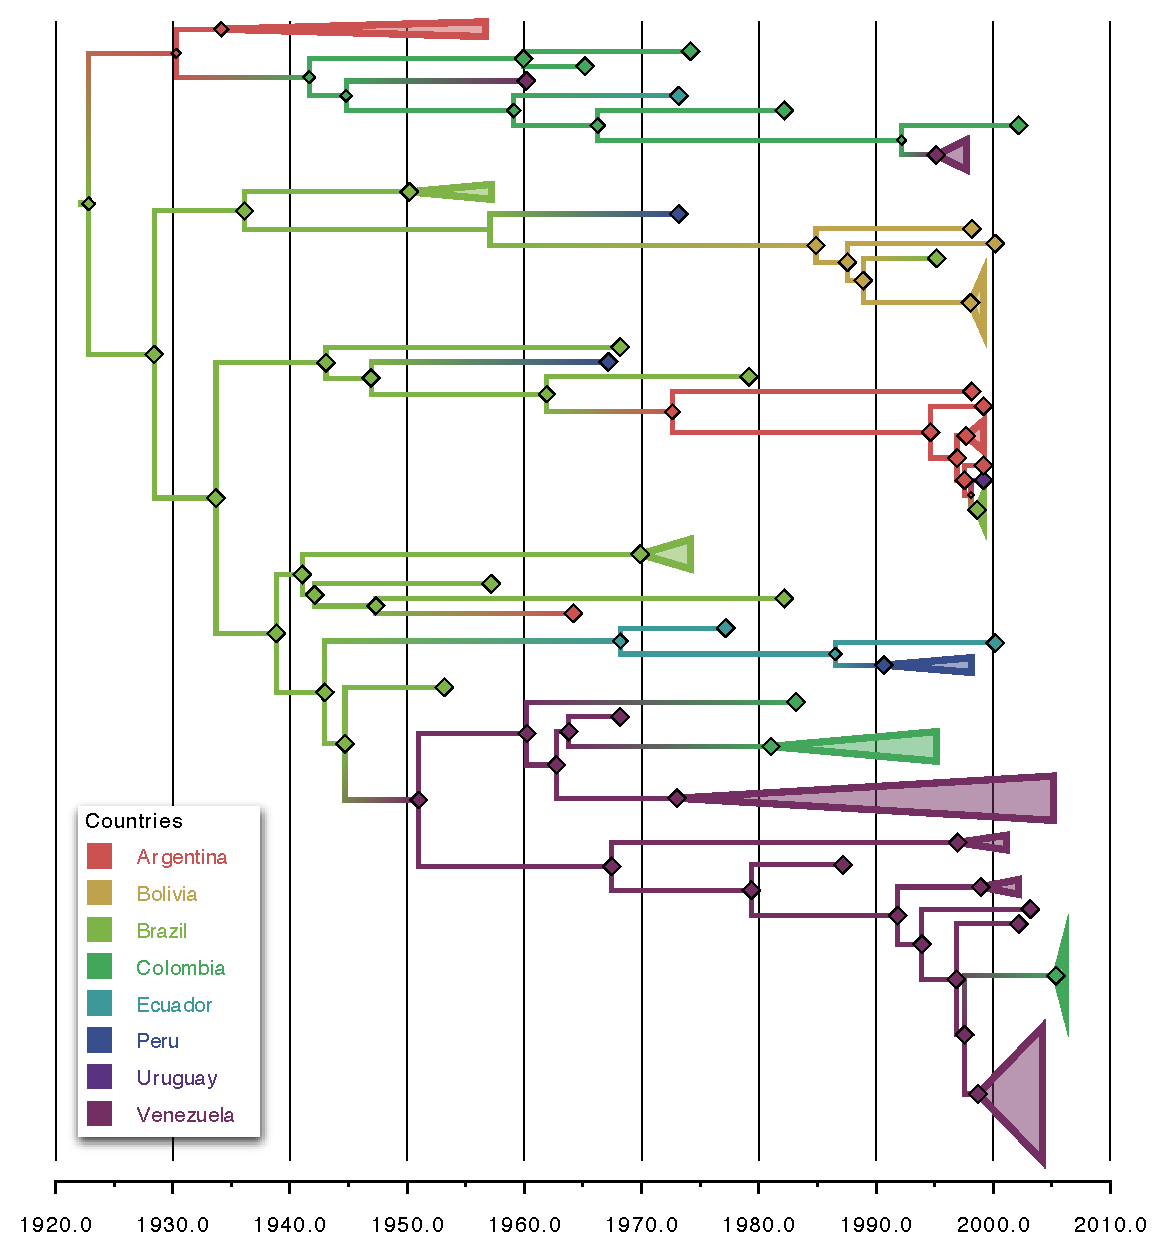
\includegraphics[width=15cm,height=10cm]{FIGURES/A.pdf}
\end{center}
\caption{
{\bf Phylogenetic Relationships of 131 serotype A FMDV isolates from South America.} Time-scaled phylogenetic maximum clade credibility (MCC) tree for FMDV VP1 sequences from eight countries in the period 1955-2010 is presented. Tips were collapsed for clarity and colored according to geographic origin. Diamonds sizes are proportional to posterior probabilities.\\
}
\label{fig:Atree}
\end{figure}
%%%%%%%%%%%%%%%%%%%%%%%%%%
%%%%%%%%%%%%%%%%%%%%%%%%%%
\newpage
\begin{figure}[!ht]
\begin{center}
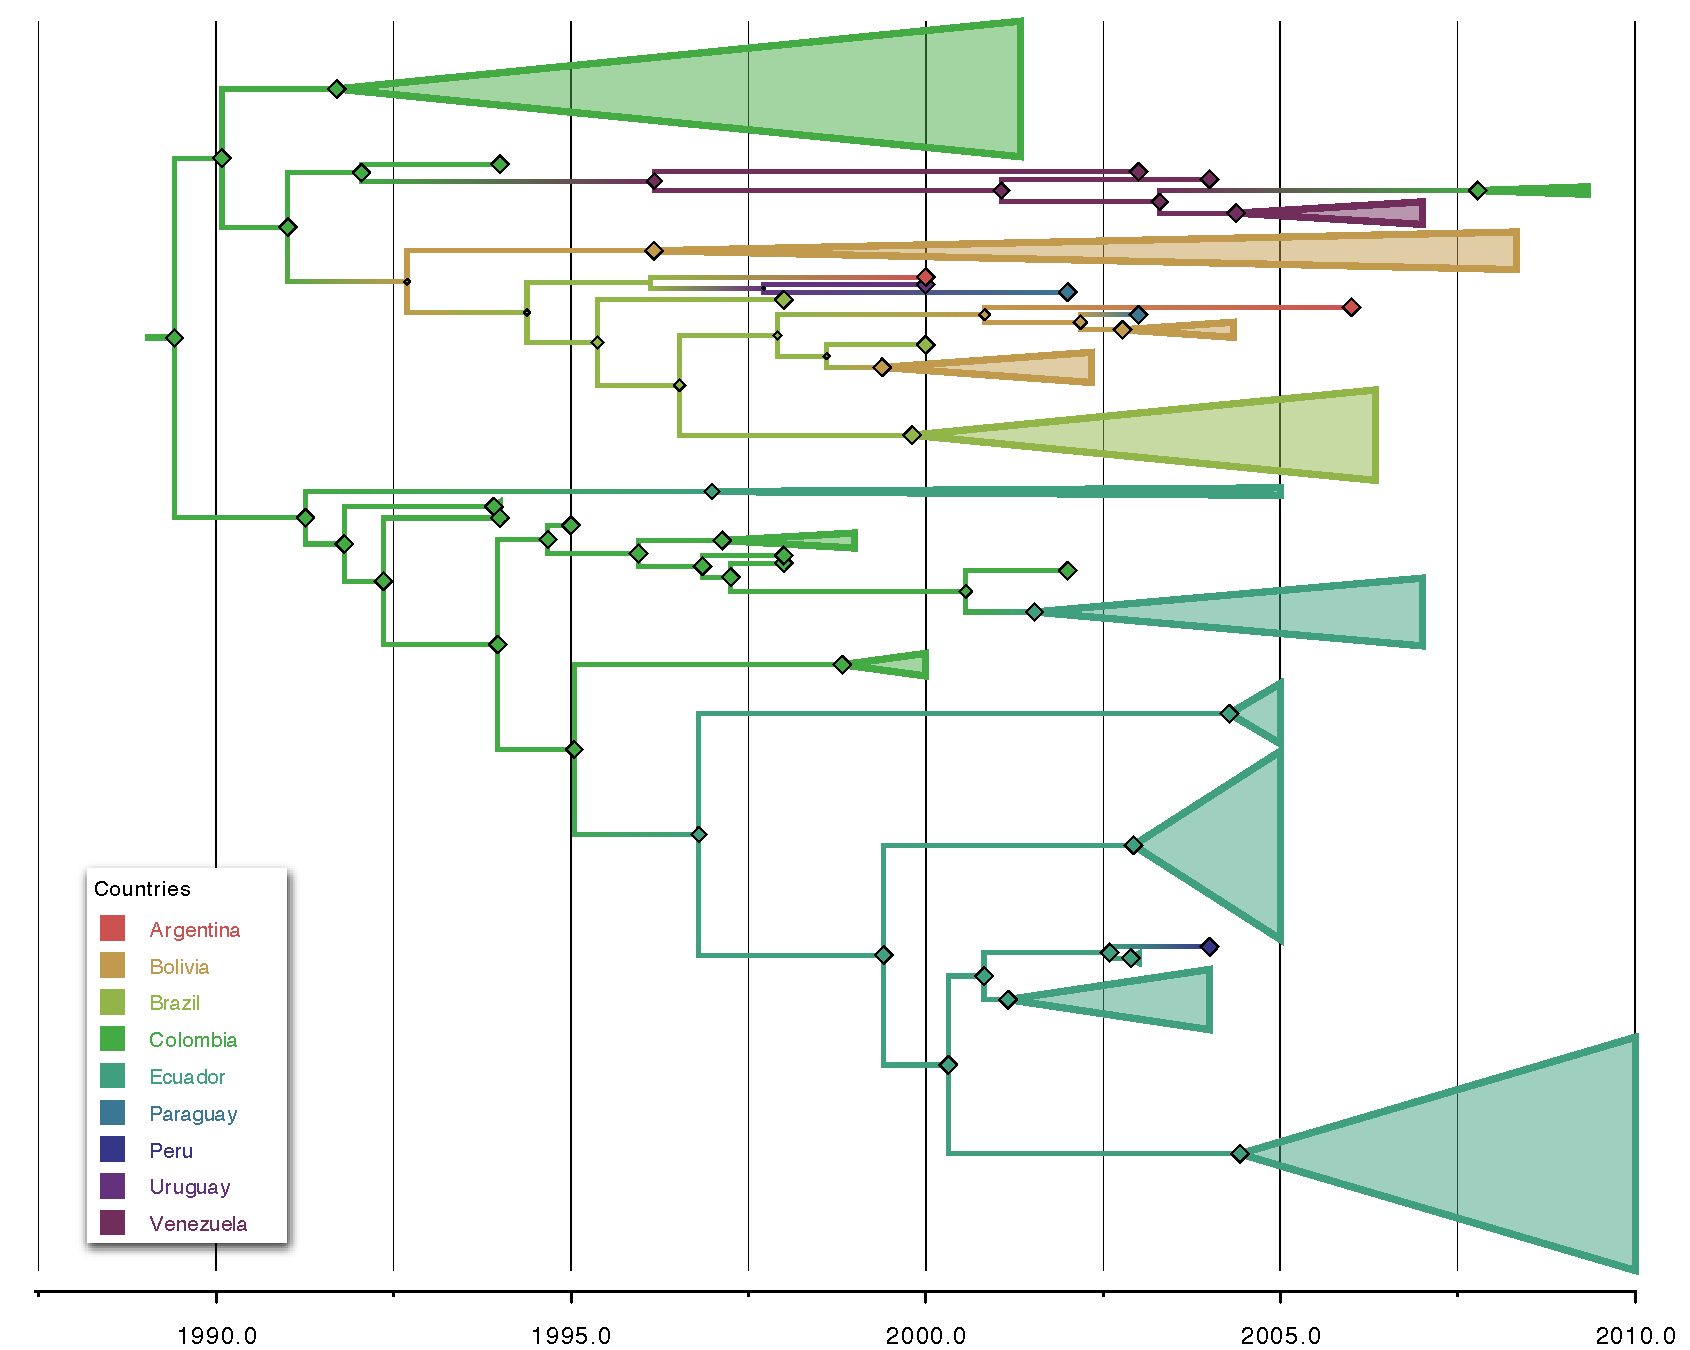
\includegraphics[width=15cm,height=10cm]{FIGURES/O.pdf}
\end{center}
\caption{
{\bf Phylogenetic Relationships of 167 serotype O FMDV isolates from South America.} Time-scaled phylogenetic maximum clade credibility tree for FMDV VP1 sequences from eight countries in the period 1955-2010. Tips were collapsed for clarity and colored according to geographic origin. Diamonds sizes are proportional to posterior probabilities.\\
}
\label{fig:Otree}
\end{figure}
%%%%%%%%%%%%%%%%%%%%%%%%%%
%%%%%%%%%%%%%%%%%%%%%%%%%%
\newpage
\begin{figure}[!ht]
\begin{center}
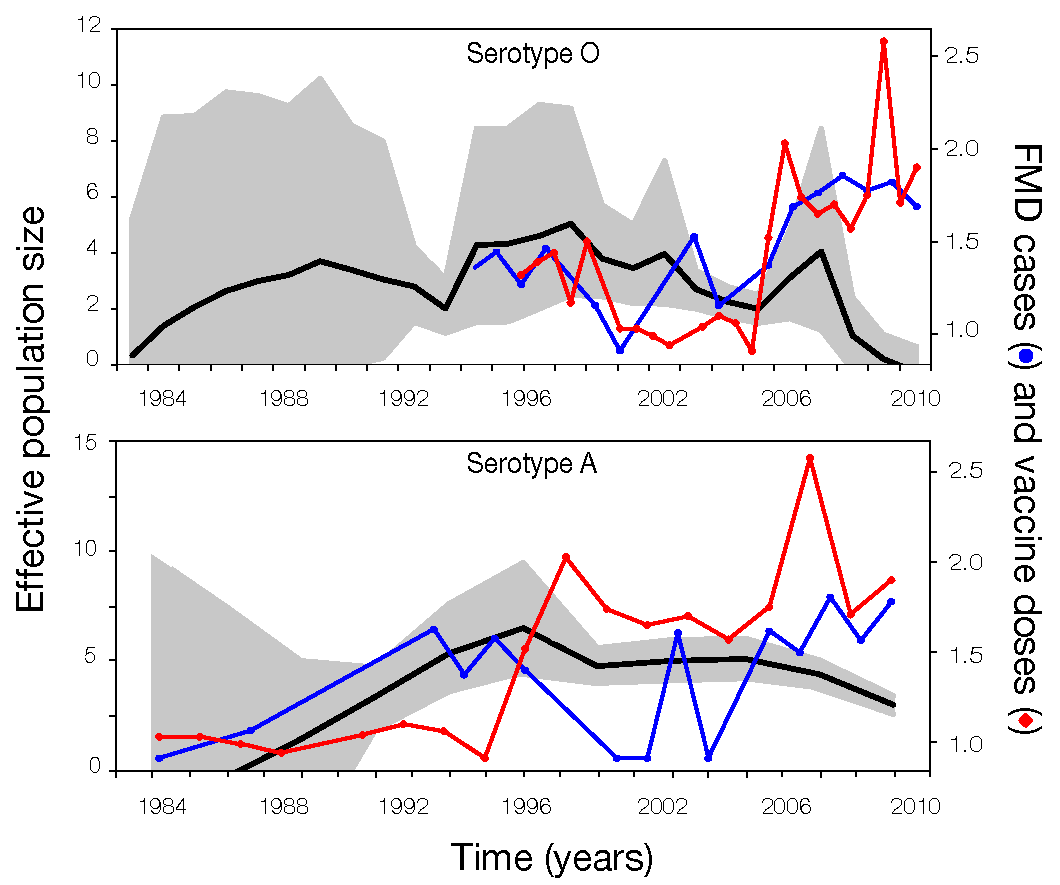
\includegraphics[width=15cm,height=15cm]{FIGURES/skygrid.pdf}
\end{center}
\caption{
{\bf Temporal dynamics of FMDV serotypes A and O in South America} Population dynamics were reconstructed for both serotypes using the Skygrid model (see Methods). Additionally, data on vaccination  (doses per head) and (log) FMD serotype-specific notifications were superimposed on the demographic reconstruction, with 95 \% Bayesian Credible Intervals shaded in grey.\\
}
\label{fig:skygrid}
\end{figure}
%%%%%%%%%%%%%%%%%%%%%%%%%%
%%%%%%%%%%%%%%%%%%%%%%%%%%

\newpage
\begin{figure}[!ht]
\begin{center}
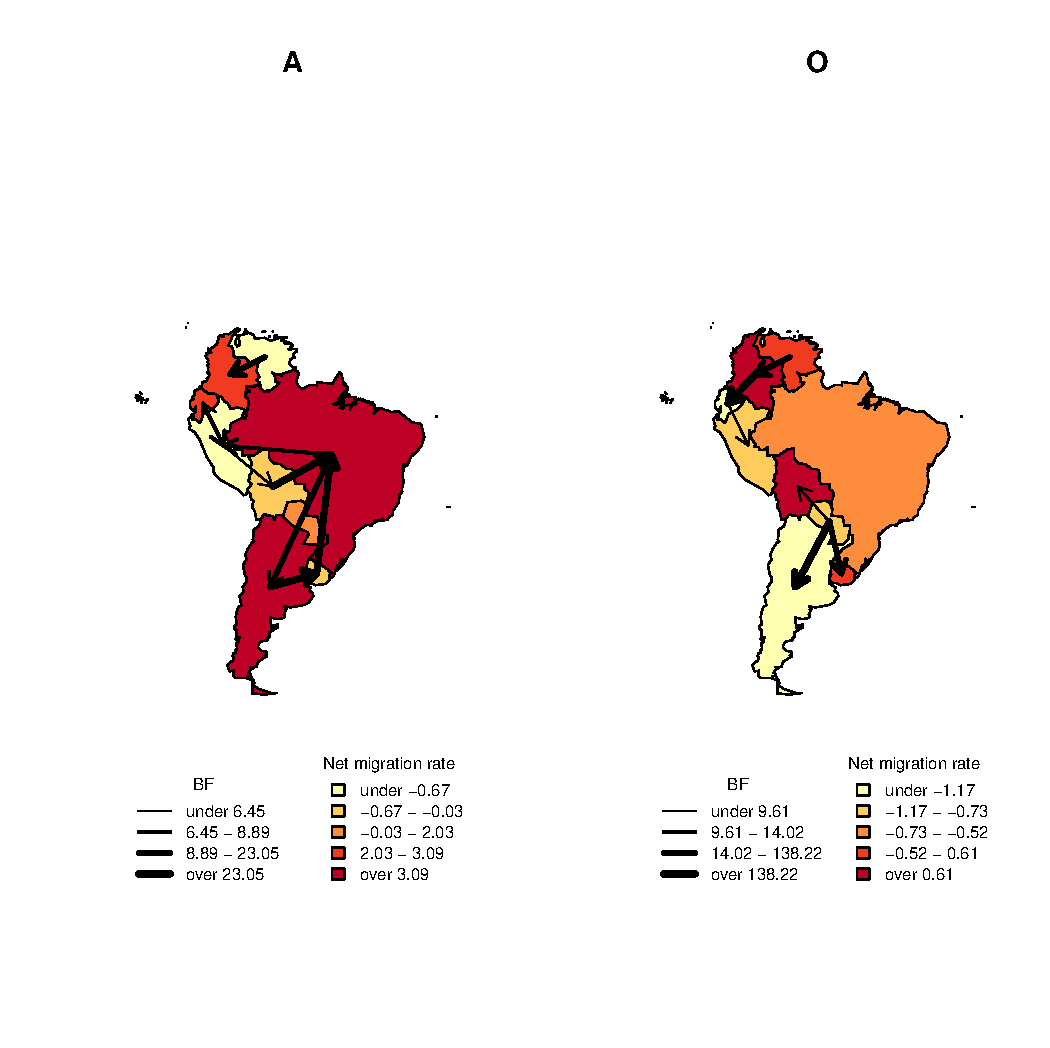
\includegraphics[width=15cm,height=15cm]{FIGURES/compound.pdf}
\end{center}
\caption{
{\bf Migration networks for FMDV serotypes A and O in South America} We estimated the number of migration events between countries using Markov jumps.  Bayesian Stochastic Variable Search Selection (BSVSS) was used to determine most significant migration routes and Bayes factors are depicted by arrows, with line thickness proportional to BF magnitude. Coroplethic maps show the net migration rates for each country, for both serotypes.\\
}
\label{fig:mj&BFs}
\end{figure}
%%%%%%%%%%%%%%%%%%%%%%%%%%
%%%%%%%%%%%%%%%%%%%%%%%%%%

\newpage
\begin{figure}[!ht]
\begin{center}
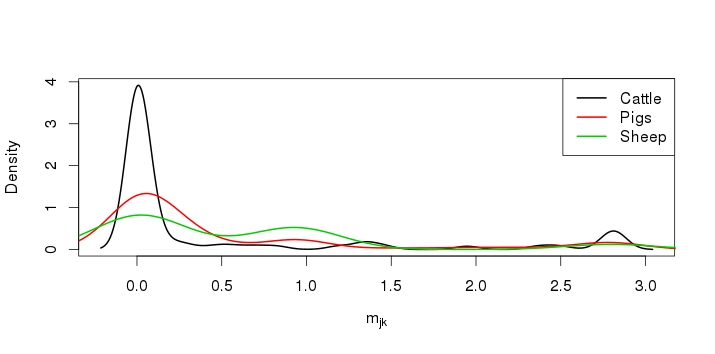
\includegraphics[width=15cm,height=15cm]{FIGURES/trade_info.jpeg}
\end{center}
\caption*{
{\bf S1. Kernel density estimation for the trade-informed priors used in this study}.\\
}

\label{sfig:tradeinfo}
\end{figure}
%%%%%%%%%%%%%%%%%%%%%%%%%%
%%%%%%%%%%%%%%%%%%%%%%%%%%

\newpage
\section*{Tables}
\begin{table}[!ht]
\caption{
\textbf{Spatial signal for serotype A.} 1-AI = association index; 2-PS = parsimony score; 3- Monophiletic clade size}
\begin{tabular}{c|c|c|c}
Statistic &	Observed mean ( 95\% CI)&	Null mean ( 95\% CI)&	p-value\\
AI$^1$	&1.56 (1.10, 2.01)& 10.75 (9.67, 11.83) &0.000\\
PS$^2$	&22.88 (22.00, 24.00)	&66.78	(63.06, 70.01)	&0.000\\
Argentina &12.31 (12.00, 14.00)	&3.45	(2.22, 5.11)	&0.001\\
MC$^3$ Brazil &10.27	(10.00, 11.00)	&2.02 (1.25, 3.00) &0.001\\
Bolivia &6.00 (6.00, 6.00)	&1.39 (1.00, 2.00)	&0.001\\
Colombia &5.11 (5.00, 6.00)	&1.10  (1.00, 1.99)	&0.001\\
Ecuador &1.00 (1.00, 1.00)	&1.00 (1.00, 1.00)	&1.000\\
Peru&1.00 (1.00, 1.00)	&1.02 (1.00, 1.00)	&1.000\\
Uruguay &5.11 (5.00, 7.00)	&1.50	(1.00, 2.03)	&0.001\\
Venezuela&1.82 (1.00, 2.00)	&1.02 (1.00, 1.08)	&0.010\\
\end{tabular}
\begin{flushleft}
\end{flushleft}
\label{tab:BaTSA}
 \end{table}
%%%%%%%%%%%%%%%%%%%%%%%%
%%%%%%%%%%%%%%%%%%%%%%%%
\begin{table}[!ht]
\caption{
\textbf{Spatial signal for serotype O. } 1-AI = association index; 2-PS = parsimony score; 3- Monophiletic clade size}
\begin{tabular}{c|c|c|c}
Statistic &	Observed mean ( 95\% CI)&	Null mean ( 95\% CI)&	p-value\\
AI$^1$ &	0.87 (0.59, 1.19)&	11.58 (10.52, 12.67)&	0.000\\
PS$^2$ &	16.23 (15.00, 17.00)&	71.23 (68.17, 73.97)&	0.000\\
MC$^3$ Ecuador& 13.00 (13.00, 13.00)&	1.34 (1.00, 2.00)&	0.001\\
Peru&	1.00 (1.00, 1.00)&	1.01 (1.00, 1.00)&	1.000\\
Colombia&	1.00 (1.00, 1.00)&	1.00 (1.00, 1.00)&	1.000\\
Venezuela&	6.00 (6.00, 6.00)&	1.28 (1.00, 2.00)&	0.001\\
Bolivia &	1.00 (1.00, 1.00)&	1.00 (1.00, 1.00)&	1.000\\
Brazil&	19.00 (19.00, 19.00)&	2.19 (1.66, 3.03)&	0.001\\
Paraguay&	39.40 (31.00, 58.00)&	4.67 (3.43, 6.39)&	0.001\\
Argentina&	1.00 (1.00, 1.00)&	1.00 (1.00, 1.00)&	1.000\\
Uruguay&	4.00 (4.00, 4.00)&	1.06 (1.00, 1.32)&	0.001\\
\end{tabular}
\begin{flushleft}
\end{flushleft}
\label{tab:BaTSO}
 \end{table}
%%%%%%%%%%%%%%%%%%%%%%%%
%%%%%%%%%%%%%%%%%%%%%%%%
\begin{table}[!ht]
\caption{
\textbf{Spatial model selection results for serotype A. } GUY's SHARE.}
\begin{tabular}{c|c|c|c|c|c}
Model & AICM  & PS    & SS    & Root  & Pr(Root)\\
    \hline
    Distance & 24147.71 & \textbf{-2545.71} & \textbf{-2553.25} & Per   & 0.94 \\
    Sheep & 24112.61 & -2547.57 & -2555.00 & Bra   & 0.83 \\
    Pig & 24149.06 & -2556.06 & -2563.27 & Col   & 0.99 \\
    Uniform & 24139.71 & -2560.88 & -2568.39 & Per   & 0.94 \\
    Cattle & 24191.77 & -2574.87 & -2578.35 & Per   & 0.92 \\
    Sheep-Freq & 24175.47 & -2579.22 & -2585.73 & Per   & 0.9 \\
    Simple & \textbf{23877.84} & -2584.48 & -2588.93 & -     & - \\
    Pig-Freq & 24271.98 & -2609.59 & -2617.82 & Col   & 0.51 \\
    Cattle-Freq & 24305.81 & -2638.48 & -2645.64 & Per   & 0.89 \\
\end{tabular}
\begin{flushleft}
\end{flushleft}
\label{tab:prootA}
 \end{table}
%%%%%%%%%%%%%%%%%%%%%%%%
%%%%%%%%%%%%%%%%%%%%%%%%
\begin{table}[!ht]
\caption{
\textbf{Spatial model selection results for serotype O. } GUY's SHARE.}
\begin{tabular}{c|c|c|c|c|c}
Model	&AICM	&PS	&SS	&Root	&Pr(Root)\\
\hline
Uniform	&15569.12	&\textbf{-8285.10}	&\textbf{-8294.49}	&Col	&0.92\\
Cattle-Freq	&15565.93	&-8286.50	&-8295.66	&Col	&0.97\\
Distance	&15542.21	&-8287.09	&-8298.13	&Col	&0.92\\
Sheep	&15585.43	&-8289.04	&-8298.31	&Col	&0.98\\
Cattle	&15548.98	&-8292.72	&-8300.47	&Col	&0.95\\
Pig	&15580.74	&-8292.14	&-8301.20	&Col	&0.52\\
Sheep-Freq	&15566.45	&-8294.83	&-8301.42	&Col	&0.86\\
Pig-Freq	&15604.59	&-8308.37	&-8315.31	&Col	&0.57\\
Simple	&\textbf{15419.93}	&-8407.13	&-8412.42	&-	&-\\
\end{tabular}
\begin{flushleft}
\end{flushleft}
\label{tab:prootO}
 \end{table}
%%%%%%%%%%%%%%%%%%%%%%%%
%%%%%%%%%%%%%%%%%%%%%%%%
\newpage
\begin{table}[!ht]
\caption*{\textbf{Table S1. Model selection for tree (coalescent) model and clock for both serotypes.}  ULN= uncorrelated log-normal; UCED = uncorrelated exponential . Best fitting models (highest log-likelihood) are highlighted in bold.}
\begin{tabular}{c|c|c|c|c|c}
Serotype	&Coalescent	&Clock	&Log-Likelihood$^{1}$\\
\hline
A	&Constant	&ULN	&-12285\\
A	&Skyride 	&ULN	&\textbf{-12274}\\
A	&Constant	&UCED	&-12316\\
A	&Skyride 	&UCED	&-12307\\
O	&Constant	&ULN	&-8087\\
O	&Skyride 	&ULN	&-8082\\
O	&Constant	&UCED	&-8090\\
O	&Skyride 	&UCED	&\textbf{-8069}\\
\end{tabular}
\begin{flushleft}
\end{flushleft}
\label{stab:treeclockselection}
 \end{table}
%%%%%%%%%%%%%%%%%%%%%%%%
%%%%%%%%%%%%%%%%%%%%%%%%
\end{document}